\documentclass[tikz]{standalone}
\usepackage{circuitikz}
\begin{document}

\usetikzlibrary{arrows.meta} 
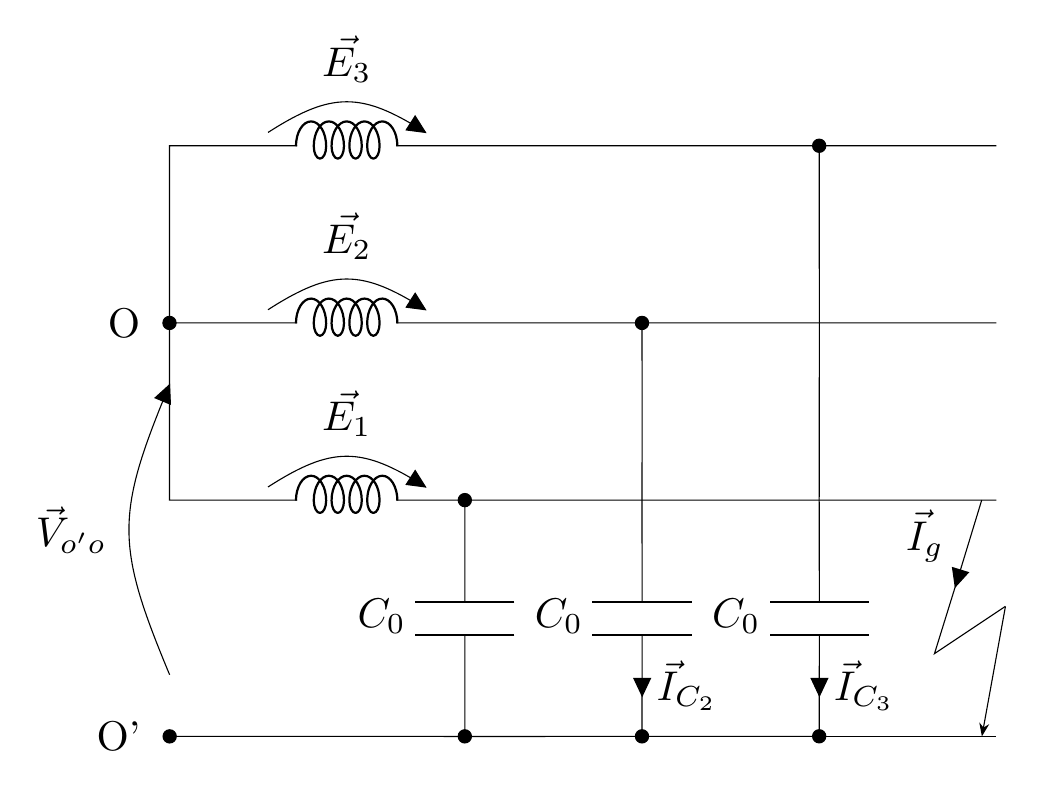
\begin{tikzpicture}[scale=1.5, transform shape]
\draw (0,0) node[label={left:O}](O){}  to[short,*-]  ++(0,1.5) -- ++(0.5,0)  to[inductor,v^={$\vec{E_3}$}] ++(2,0) -- ++(3,0) node(V3){} -- ++(1.5,0);
\draw (O.center) -- ++(0.5,0) to[inductor,v^={$\vec{E_2}$}] ++(2,0) -- ++(1.5,0) node(V2){} -- ++(3,0);
\draw (O.center) |- ++(0.5,-1.5) to[inductor,v^={$\vec{E_1}$}] ++(2,0)  node(V1){}-- ++(4.5,0) node(shock){};

\draw (V1.center) to[C,l_=$C_0$,*-*] ++(0,-2);
\draw (V2.center) to[short,*-] ++(0,-1.5) to[C,l_=$C_0$,-*,i=$\vec{I}_{C_2}$] ++(0,-2);
\draw (V3.center) to[short,*-] ++(0,-3) to [C,l_=$C_0$,-*,i=$\vec{I}_{C_3}$] ++(0,-2) node(V0){};

\draw (V0.center) -- ++(1.5,0) node(gnd){};
\draw (V0.center) to [short,-*] ++(-5.5,0) node[label={left:O'}](O'){};
\draw (O') to[open,v^=$\vec{V}_{o'o}$] (O);

\draw (shock.west) to[short,i_=$\vec{I}_g$] ++(-0.4,-1.3) -- ++(0.6,0.4) node(arr_start){};
\draw  [-Stealth](arr_start.center) -- (gnd.west);
\end{tikzpicture}

\end{document}